\documentclass[12pt,fleqn]{article}\usepackage{../../common}
\begin{document}
ID3 Karar Ağacı

Zeki arama yazısında, arama algoritmasına tahmin yeteneği kazandırdığımızda
problem sonucuna ulaşım hızını arttırmıştık. Tahmin yeteneği oyun tahtasına
değer biçebilen işlev sayesinde bilgisayara kodlanmıştı.

Bir soru; İnsan zekasında tahmin neye dayanır? Üzerinde bilgimiz,
tecrübemiz olmayan konu hakkında tahmin yapabilirmiyiz? Hayır. Öyleyse
bilgisayara tahmin özelliği kazandırdığımız zaman aynı zamanda makinaya
"bilgi" verdiğimizi söyleyebiliriz. Makinayı bilgilendirdik, ona tecrübe
kazandırdık da diyebiliriz çünkü tahmin, bir konu hakkında bilgimize,
tecrübemize dayandığı ölçüde başarılı olabilir.

Bilgisayara bilgiyi iki şekilde verebiliriz: Yapısal, ya da işlevsel. Zeki
arama örneği işlevsel bir örnek gösterdi. Bilgiyi, bilgisayara algoritma
halinde verdik. Tahta değerlendiren işlev, her taşa göre nasıl hesap
yapacağını biliyordu. Bu hesabı toplama ve çarpma işlemlerini kullanarak ve
daha önceden "bildiği" ağırlıklara göre birbirine ekleyerek tahta hakkında
ne düşündüğünü tek bir sayı halinde bildirdi, ve algoritmanın geri kalanı
bu değerler ile doğru seçimi yaparak sonuca ulaştı.

Bu yazıda oyun oynama yerine birçok seçeneğin arasında karar vermek
konusunu işleyeceğiz. Zeki aramanın aksine bilgi bilgisayara işlev olarak
değil, bir karar ağaç yapısı olarak verilecek, ve daha da iyisi
bilgisayarın bu yapıyı "örnek veriden" kendi kendine öğrenmesi
sağlanacak.

Karar Ağacı Nedir?

Video, televizyon gibi bir ev elektronik eşyasının kılavuzunda "şu, şöyle
olduysa şöyle yap" gibi tarifler vardir. İlk önce kontrol edilmesi tavsiye
edilen ayarlar vardır, ve bu ayarlardan gelen cevaba göre değişik ayarlara
bakılması tavsiye edilir ve en sonunda kılavuz ne hangi özel düğmeye
basılması gerektiğini söyler. Kullanım kılavuzları onlarca sayfalık bir
karar ağacıdır denebilir. İnsanlara karar ağacın kavramı doğal geldiği için
kılavuzlar bu şekilde hazırlanmıştır.

Diğer bir örnek, lokantalarda çok yemek yiyen birisinin kullandığı karar
ağacı olabilir. Bu kimse her türlü değişik şart altında değişik lokantalara
gitmiş, ve her seferindeki memnuniyet/pişmanlık durumunu kayıt ederek bir
karar ağacı oluşturmuş ise, artık yeni bir lokantada karar kılması için
kapısından şöyle içeri bakıp menüye göz gezdirmesi yeterli olacaktır. Bu
kişinin lokanta deneyimleri mesela aşağıdaki gibi kayıtlı olsun.

\begin{minted}[fontsize=\footnotesize]{python}
labels = ['BASKA','BAR','HAFTASONU','ACMIYIZ','MUSTERILER',\
'FIYAT','YAGMUR', 'RESERVASYON','YEMEKTURU','BEKLEMESURESI','BEKLEYELIM']
dataSet = [
['EVET','HAYIR','HAYIR','EVET','BIRAZ','DDD','HAYIR','EVET','FRANSIZ','0','EVET'],
['EVET','HAYIR','HAYIR','EVET','DOLU','D','HAYIR','HAYIR','TAYLAND','30','HAYIR'],
['HAYIR','EVET','HAYIR','HAYIR','BIRAZ','D','HAYIR','HAYIR','KEBAP','0','EVET'],
['EVET','HAYIR','EVET','EVET','DOLU','D','EVET','HAYIR','TAYLAND','10','EVET'],
['EVET','HAYIR','EVET','HAYIR','DOLU','DDD','HAYIR','EVET','FRANSIZ','60','HAYIR'],
['HAYIR','EVET','HAYIR','EVET','BIRAZ','DD','EVET','EVET','ITALYAN','0','EVET'],
['HAYIR','EVET','HAYIR','HAYIR','HIC','D','EVET','HAYIR','KEBAP','0','HAYIR'],
['HAYIR','HAYIR','HAYIR','EVET','BIRAZ','DD','EVET','EVET','TAYLAND','0','EVET'],
['HAYIR','EVET','EVET','HAYIR','DOLU','D','EVET','HAYIR','KEBAP','60','HAYIR'],
['EVET','EVET','EVET','EVET','DOLU','DDD','HAYIR','EVET','ITALYAN','10','HAYIR'],
['HAYIR','HAYIR','HAYIR','HAYIR','HIC','D','HAYIR','HAYIR','TAYLAND','0','HAYIR'],
['EVET','EVET','EVET','EVET','DOLU','D','HAYIR','HAYIR','KEBAP','30','EVET']
]
\end{minted}

Peki bu veriye bakarak karar ağacını nasıl oluşturacağız?

İnsanın aklında karar ağacını oluşturması başka bilim dalları altında
araştırılıyor. Bilgisayar için karar ağacını "kendi kendine çıkartan" bir
yapay zeka algoritması (ID3), bu yazımızın konusu olacak. ID3 ve genelde
öğrenen algoritmalar ve ileride mekanize-öğrenme konusuna giriş açısından
yararlı olabilir, ve bu konuda zaten en popüler yaklaşım olan ID3'ün geniş
bir uygulama alanı vardır.

Algoritma

Karar ağacımız öyle olsun ki, eğitim verisi ile eğitildikten sonra, yeni
bir soruya karşılılk, üstten başlayarak yeni şartlar çerçevesinde (ama eski
veriye göre kurulmuş) ağaçta bizi bir 'evet' ya da 'hayır' cevabına doğru
yönlendirsin. İyi kurulmuş bir karar ağacı, "en az" soru ile "en çabuk"
cevaba erişmemizi sağlayan ağaçtır. Çünkü ileride de göreceğimiz gibi, aynı
veri için birden fazla değişik karar ağacı kurmak mümkündür.

Evet, algoritmamıza başlayalım. Veriyi bölmek için, bir başlık seçmemiz
gerekiyor. Bu seçimi şimdilik rasgele yapalım, diyelim ki "Müşteri"
başlığını seçtik. Veriye bakınca, bu başlık altında "Hiç", "Biraz" ya da
"Dolu" değerlerini görüyoruz. Bu başlığı en üst düğüm olarak ağaca
yerleştirelim, ve veriyi, bu başlığın tekrar eden değerlere göre
guruplayıp, bölelim.

Alttaki ağaç, müşteri başlığı üzerinden oluşturulan ağacımızın ilk
seviyesidir.

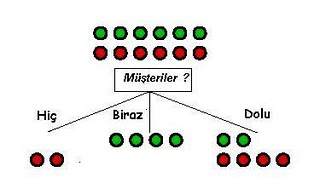
\includegraphics[height=5cm]{id3_hangi_baslik_1.jpg}

Yeşil ve kırmızı toplar evet=yeşil, hayır=kırmızı cevaplarını temsil
ediyorlar. Resimin anlatmak istediği, karar ağacı öğreniminin, eğitim
verisinin tamamını böldüğü, ve seçenekler arasında taksim
ettiği. Elimizdeki verinin "hedef başlığı" "bekleyelim mi?" sorusudur, ve
cevabı sadece evet ya da hayır olabilir. Yazının geri kalan kısmında
kırmızı ve yeşil topların hepsini göstermeyeceğiz. Kolaylık bakımından
ağacın en uç kısmında tamamen yeşil ya da tamamen kırmızı var ise tek bir
renk göstermek yeterli olacak.

Ağacın bu ilk seviyesine bakınca, görüyoruz ki daha şimdiden elimizde
yararlı bir karar ağacı var. Çünkü eğer, 'müşteriler' sorusuna yeni sorunun
cevabı "hiç" olsaydı, direk olarak bir "Y" (Yanlış) cevabına erişmemiz
mümkün oluyordu. Bu noktada iş bitiyor, karar verilmiş olurdu. Tabii bu
cevap senaryosu çok iyimser bir senaryodur, çünkü eğer yeni sorunun cevabı
"Dolu" olsa idi, bu dalı izleyerek hala bölünmüş olan bir dala geldiğimizi
görecektik. Demek ki ağaç oluşturan algoritmanın işi daha bitmedi. "Dolu"
dalını takip ederek, oradaki verileri de bölmeye devam etmemiz gerekiyor.

Bu dalı bölmek için, 'müşteriler' başlığından sonra, gene rasgele olarak,
'bekleme süresi' başlığını seçebiliriz. Eğer lokanta dolu ise, kapıda
beklememiz için eğitim verisinde elimizde olan bekleme süreleri bu başlık
altında toplanmış. Mümkün değerler 60 dakika'dan fazla, 30-60 dakika arası,
10-30 dakika arası, ya da 10 dakikadan daha az beklemek olarak
görülüyor. Bu bölünmeyi de yaptıktan sonra, sırası ile ``müşteriler=dolu''
ve ``bekleme süresi=60 dakidan fazla'' sorusunun bizi kesin bir cevaba
eriştirdiğini göreceğiz. Ayrıca, ``müşteriler=dolu'' ve ``10 dakikadan az
beklemek'' sorusu bizi 'evet' cevabına getirecektir. Bunlar da güzel. Fakat
işimiz daha bitmedi, halâ bölünmemiş dallar var, vs.

Herhalde algoritmanın bölen ve ağaç oluşturan kısmının mantığı
anlaşıldı. Tahmin edilecegi gibi bu bölme ve dal oluşturma işlemi tamamen
'evet' ve 'hayır' sonuçlarına erişinceye kadar devam edecek. Sonuç karar
ağacını aşağıda görüyoruz.

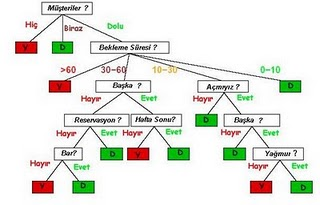
\includegraphics[height=9cm]{id3_agac_ilk.jpg}

Optimizasyon

Yapay zeka dalında, algoritmaların doğruluğu kadar, bilgisayara getirdiği
yükün ne kadar önemli olduğunu görmüştük. O kadar ki, eğer bu yük kontrol
edilir bir ölçüde değil ise, algoritmanın işe yararlılığı sorgulanmaya
başlanır. Test olarak, bir algoritmanın 12 veri satırı (yukarıdaki örnek)
yerine , 500,000 satırlık veri ile ne yapacağını sormak yerinde olur. Çünkü
insan beyninin yaptığı binbir türlü teknik kullanarak bu kadar veriyi
işlemektir, aktif zekamızda farkında olmasak bile, belli bir seviyede bu
işlemler olmaktadır. Basit bir iş gibi görünen bir yerden bir yere kalkıp
yürümek için kullandığımız algoritmaların neler çözmek zorunda olduğunu,
robot yazılımlar ile uğraşanlar bilir.

O yüzden, ID3 algoritmasını 500,000 satırlık veriyi idare edebilecek
şekilde ilerletmemiz gerekiyor.

Başlık Seçimi

Ilerletme için uygun bir zaman herhalde başlık seçimi esnâsında
olacaktır. İlk karar ağacında gördüğümüz gibi bazı sorulara olan cevaplar
daha ilk seviyede kesin cevaba erişebiliyordu. Demek ki, sürekli olarak
"uygun başlığı uygun zamanda" seçersek, ağacımızı oldukça küçültmemiz
mümkün olur. Böylece kesin cevaba erişmemiz kolaylaşır. Tabii kolaylık
derken, 500,000 satırlık veri için 100 derinliğindeki bir ağaç ile 10 birim
arasındaki bir farktan bahsediyorum, ki bu fark hiç yabana atılacak bir
fark değildir.

Peki uygun başlık nedir? Mesela ilk seviye için, müşteri yerine, "yemek
türü" başlığını seçseydik, daha mı iyi bir seçim yapmış olurduk? Bu farazi
bölünmeyi aşağıdaki şekilde görelim.

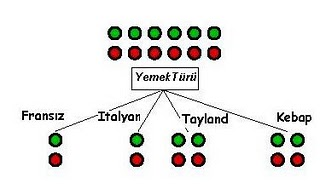
\includegraphics[height=5cm]{id3_hangi_baslik_2.jpg}

Görüyoruz ki, bu yeni bölünme bizi hiç bir kesin cevaba götürmedi. Üstüne
üstlük, bütün bu dalların alt-dalları, onlarında alt-dalları derken
ağacımızın arap saçına dönmesi ihtimal dahilinde. Demek ki 'yemek türü'
bölünmesi bize yeni "bilgi" sâğlamadı. Halâ elimizde kesin cevaplar değil,
seçenekler var.

Bize öyle bir işlev lazım ki, her parçaya bakıp kazandırdığı bilgiyi
ölçsün, hala bölünmüş kalan kısımlar içinde bile, onlardan en iyi olanını
seçsin. İşte bu noktada bilgi kuramı yardımımıza yetişiyor.

Bilgi Kuramı

Bilgi kuramı (information theory), bilgiyi nasıl kodlayacağımızı ve sonuç
kodlamanın ne kadar yer tutacağı gibi sorunlar ile uğraşır. Mesela,
elimizde 2 değişik değer var ise ve bu değerleri ikili düzende kodlamamız
gerekse, bu iş için kaç tane bit gerekir?

Cevap: Bir tane.

Peki, 4 tane değer olduğunu düşünelim. Şimdi kaç tane? Cevap: İki. Tekrar
eden mantık belki farkedilmistir; eğer "kaç bit" sorusu ile "eldeki
bilgi" arasında matematiksel bir bâglantı kurmak gerekse (K ye B), şöyle
yazabiliriz. Parça Bilgi Değeri şuna eşit:

$$ -\frac{d}{d+y} \log_2 \bigg( \frac{d}{d+y} \bigg) - 
\frac{y}{d+y} \log_2 \bigg( \frac{y}{d+y} \bigg) 
$$

Adresleme, onluk düzen ve ikilik düzen arasında gidip gelme gibi
problemlerden hatırlayabileceğimiz bir sonuç bu. Ya da, 'iki tane bit en
fazla kaç onluk sayıyı gösterir' sorusunun tersten sorulmuş şeklidir
denebilir.

Şimdi bu ters soruyu karar ağacının böldüğü her parçaya soralım. Tabii
birkaç değişiklik yapmamız gerekecek. Mesela elimizde
\verb!yemekturu=tayland! sonucunda tek bir parça üzerine 2 yanlış ve 2
doğru değer var ise, bu düğümün bilgi değerini kesirler ile hesaplamamız
gerekecek. Kesirler ile uğraşırken log işlevi eksi değerler getireceği için
cevabı önce kesirin kendisi, sonra da eksi ile çarpmamız lazım ($\log$, 0
ve 1 arası için eksi değer getirir). Yani, genel olarak iki cevaplı bir
uzayda, tek parçanın bilgi değeri şöyle gösterilebilir. Parça Bilgi Değeri
suna eşit:

$$ B(O(v_1),...,O(V_n)) = \sum_{i=1}^{n} -O(v_i)\log_2O(v_i) $$

$O$, olasılığı temsil ediyor. 

Genel olarak göstermek gerekirse, n cevaplı bir uzayda parçanın bilgi
değeri şudur. 

$$ B \bigg(\frac{1}{2}, \frac{1}{2} \bigg) = 
\frac{1}{2}\log_2 \bigg(\frac{1}{2} \bigg) 
- \frac{1}{2}\log_2 \bigg(\frac{1}{2} \bigg) = \textrm { 1 bit }
 $$

Formülü kontrol etmek için, başta verdiğimiz bit örneğini kullanalım: 2
değişik değer için kaç bit gerekir?

$$ \sum_{i=1}^{parca} \frac{d_i + y_i}{d+y} 
\bigg( \frac{d_i}{d_i+y_i}, \frac{y_i}{d_i+y_i} \bigg)
$$

$d_i$: i'inci parça doğru sayısı

$y_i$: i'inci parca yanlis sayisi

$d$: tüm doğrular

$y$: tüm yanlışlar

1 bit gerektiğini halâ bulabiliyoruz.

Parçaların Bilgi Değer Toplamı

Bölündükten sonra elimize geçen parçaların bilgi değer toplamı için 

Müşteri Parçaları

$$  
\frac{2}{12}B(0,1) + \frac{4}{12}B(1,0) + \frac{6}{12} B(\frac{2}{6},
\frac{4}{6}) = 0.459
$$

Yemek Türü Parçaları

$$ 
\frac{2}{12}B(\frac{1}{2},\frac{1}{2}) + 
\frac{2}{12}B(\frac{1}{2},\frac{1}{2}) + 
\frac{4}{12}B(\frac{2}{4},\frac{2}{4}) + 
\frac{4}{12}B(\frac{2}{4},\frac{2}{4}) 
= 1
 $$

Problemi sözel olarak biraz daha berraklaştıralım. Herhangi bir düğümde
iken, bu düğümün bilgi değerini B() ile bulabiliriz. Lokanta örneğinin ilk
seviyesinde, en üst düğümün bilgi değeri '1' olduğunu görülebilir, çünkü
elimizde tek düğüm, 6 yanlış, 6 doğru cevap var. Güzel.

Şimdi bir seviye aşağı inelim. Her başlığı teker teker deneyip, ve veriyi
her başlık için geçici olarak parçalayıp, muhtemel her bölünme için bu
başlığa tekâbül eden parçaların bilgi değerini toplayalım (bir üstteki
formül).

Örnek veri üzerinde üstteki formülü deneyelim (1. seviye parçalanması için)

Müşteri Parçaları

$$ 
\frac{2}{12}B(0,1) +
\frac{4}{12}B(1,0) +
\frac{6}{12}B(\frac{2}{6}, \frac{4}{6}) = 0.459
 $$

Yemek Türü Parçaları

$$ 
\frac{2}{12}B(\frac{1}{2}, \frac{1}{2}) + 
\frac{2}{12}B(\frac{1}{2}, \frac{1}{2}) + 
\frac{4}{12}B(\frac{2}{4}, \frac{2}{4}) + 
\frac{4}{12}B(\frac{2}{4}, \frac{2}{4})  = 1
 $$

Görüyoruz ki, ağacın en üst seviyesini temsil etmek için 1 bit gerekiyor
iken, müşteri bölünmesinden sonra 0.459 bit yetiyor (daha az). Fakat yemek
türü bölünmesinden sonra halâ 1 bit lâzım! Yani, yemek türü bölünmesi bize
hiç bir şey kazandırmadı.

Kazanç kelimesini aritmetik olarak şöyle târif edebiliriz: Bir düğümün
bilgi değerinden, bu düğümün alt-parçalarının bilgi değer toplamının
düşülmesi kazanç değerini verir. ID3 algoritması, tabii ki daha az bit
gerektiren ya da, daha çok bilgi "kazandıran" seçeneği takip ederse daha
etkili olur. Böylece her seviyede gitgide daha berraklaşan karar ağacı, "en
az" seviyede, kesin kararlara "en çabuk" şekilde ulaşan karar ağacı
olacaktır.

Eğer B() işlevinin iç mekanizmaları hala anlaşılmadı ise, şunları bilmek
yardımcı olabilir:

Parça tamamen yanlış değerler içeriyor (kesin cevap) = B(0,1) = 0 bit

Parça tamamen doğru değerler  içeriyor (kesin cevap) = B(1,0)  = 0 bit

...   3 doğru, 3 yanlış = B(3,3)  = 1 bit 
...   2 doğru, 4 yanlış = B(2,4)  = 0.92 bit 
...   1 doğru, 5 yanlış = B(1,5)  = 0.65 bit 

Yeni algoritmanın sonucu ortaya çıkacak karar ağacı şöyle olacaktır. Bu
ağacın ilk baştaki ağaca kıyasla çok daha küçük olduğunu görüyoruz.

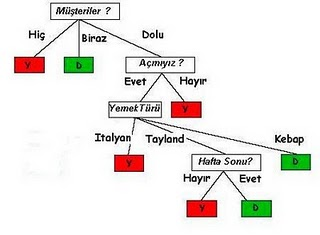
\includegraphics[height=7cm]{id3_agac_eniyi.jpg}

Kodu Python ile göstermek gerekirse [1]

\begin{minted}[fontsize=\footnotesize]{python}
from math import log
import operator

def calcShannonEnt(dataSet):
    numEntries = len(dataSet)
    labelCounts = {}
    # kac ozgun deger var ve bu degerler kac kere ortaya cikiyorlar
    for featVec in dataSet: 
        currentLabel = featVec[-1]
        if currentLabel not in labelCounts.keys(): labelCounts[currentLabel] = 0
        labelCounts[currentLabel] += 1
    shannonEnt = 0.0
    for key in labelCounts:
        prob = float(labelCounts[key])/numEntries
        shannonEnt -= prob * log(prob,2) #log base 2
    return shannonEnt
    
def splitDataSet(dataSet, axis, value):
    retDataSet = []
    for featVec in dataSet:
        if featVec[axis] == value:
            reducedFeatVec = featVec[:axis]     
            reducedFeatVec.extend(featVec[axis+1:])
            retDataSet.append(reducedFeatVec)
    return retDataSet
    
def chooseBestFeatureToSplit(dataSet):
    numFeatures = len(dataSet[0]) - 1      
    baseEntropy = calcShannonEnt(dataSet)
    bestInfoGain = 0.0; bestFeature = -1
    # tum ozellikleri ziyaret et
    for i in range(numFeatures):        
        featList = [example[i] for example in dataSet]
        uniqueVals = set(featList)       
        newEntropy = 0.0
        for value in uniqueVals:
            subDataSet = splitDataSet(dataSet, i, value)
            prob = len(subDataSet)/float(len(dataSet))
            newEntropy += prob * calcShannonEnt(subDataSet)     
        # enformasyon kazancini hesapla, yani entropideki azalisi
        infoGain = baseEntropy - newEntropy     
        # bu hesabi simdiye kadarki en iyi kazancla karsilastir
        if (infoGain > bestInfoGain):       
            bestInfoGain = infoGain         
            bestFeature = i
    return bestFeature                      


def createTree(dataSet,labels):
    classList = [example[-1] for example in dataSet]
    if classList.count(classList[0]) == len(classList): 
        # tum siniflar esitse bolmeyi durdur
        return classList[0]
    if len(dataSet[0]) == 1: 
        return majorityCnt(classList)
    bestFeat = chooseBestFeatureToSplit(dataSet)
    bestFeatLabel = labels[bestFeat]
    myTree = {bestFeatLabel:{}}
    del(labels[bestFeat])
    featValues = [example[bestFeat] for example in dataSet]
    uniqueVals = set(featValues)
    for value in uniqueVals:
        #copy all of labels, so trees don't mess up existing labels
        subLabels = labels[:]       
        myTree[bestFeatLabel][value] = \
            createTree(splitDataSet(dataSet, bestFeat, value),subLabels)
    return myTree                            

def getNumLeafs(myTree):
    numLeafs = 0
    firstStr = myTree.keys()[0]
    secondDict = myTree[firstStr]
    for key in secondDict.keys():
        if type(secondDict[key]).__name__=='dict':
            numLeafs += getNumLeafs(secondDict[key])
        else:   numLeafs +=1
    return numLeafs

def getTreeDepth(myTree):
    maxDepth = 0
    firstStr = myTree.keys()[0]
    secondDict = myTree[firstStr]
    for key in secondDict.keys():
        if type(secondDict[key]).__name__=='dict':
            thisDepth = 1 + getTreeDepth(secondDict[key])
        else:   thisDepth = 1
        if thisDepth > maxDepth: maxDepth = thisDepth
    return maxDepth

def plotNode(nodeTxt, centerPt, parentPt, nodeType):
    createPlot.ax1.annotate(nodeTxt, xy=parentPt,  xycoords='axes fraction',
             xytext=centerPt, textcoords='axes fraction',
             va="center", ha="center", bbox=nodeType, arrowprops=arrow_args )
    
def plotMidText(cntrPt, parentPt, txtString):
    xMid = (parentPt[0]-cntrPt[0])/2.0 + cntrPt[0]
    yMid = (parentPt[1]-cntrPt[1])/2.0 + cntrPt[1]
    createPlot.ax1.text(xMid, yMid, txtString, \
                        va="center", ha="center", rotation=30)

def plotTree(myTree, parentPt, nodeTxt):
    numLeafs = getNumLeafs(myTree)  
    depth = getTreeDepth(myTree)
    firstStr = myTree.keys()[0]     
    cntrPt = (plotTree.xOff + (1.0 + float(numLeafs))/2.0/plotTree.totalW,\
              plotTree.yOff)
    plotMidText(cntrPt, parentPt, nodeTxt)
    plotNode(firstStr, cntrPt, parentPt, decisionNode)
    secondDict = myTree[firstStr]
    plotTree.yOff = plotTree.yOff - 1.0/plotTree.totalD
    for key in secondDict.keys():
        if type(secondDict[key]).__name__=='dict':
            plotTree(secondDict[key],cntrPt,str(key))        
        else:  
            plotTree.xOff = plotTree.xOff + 1.0/plotTree.totalW
            plotNode(secondDict[key], (plotTree.xOff, plotTree.yOff), \
            cntrPt, leafNode)
            plotMidText((plotTree.xOff, plotTree.yOff), cntrPt, str(key))
    plotTree.yOff = plotTree.yOff + 1.0/plotTree.totalD

def createPlot(inTree):
    fig = plt.figure(1, facecolor='white')
    fig.clf()
    axprops = dict(xticks=[], yticks=[])
    createPlot.ax1 = plt.subplot(111, frameon=False, **axprops)    
    plotTree.totalW = float(getNumLeafs(inTree))
    plotTree.totalD = float(getTreeDepth(inTree))
    plotTree.xOff = -0.5/plotTree.totalW; plotTree.yOff = 1.0;
    plotTree(inTree, (0.5,1.0), '')
    plt.savefig('id3_1.png')

decisionNode = dict(boxstyle="sawtooth", fc="0.8")
leafNode = dict(boxstyle="round4", fc="0.8")
arrow_args = dict(arrowstyle="<-")

tree = createTree(dataSet, labels)
createPlot(tree)
\end{minted}

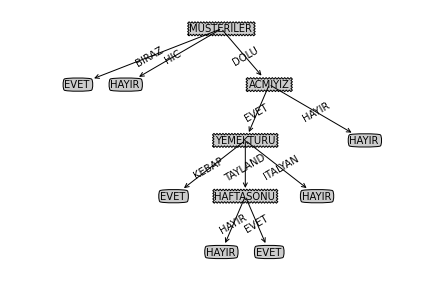
\includegraphics[height=10cm]{id3_1.png}

Aynı kodu LİSP ile görelim,

\inputminted[fontsize=\footnotesize]{python}{id3.lisp}

\begin{minted}[fontsize=\footnotesize]{python}
!clisp id3.lisp
\end{minted}

\begin{verbatim}
MUSTERILER
 = BIRAZ => EVET
 = DOLU
     ACMIYIZ
      = EVET
          YEMEKTURU
           = TAYLAND
               HAFTASONU
                = HAYIR => HAYIR
                = EVET => EVET
           = ITALYAN => HAYIR
           = KEBAP => EVET
      = HAYIR => HAYIR
 = HIC => HAYIR

"Tamam. Birim Testler Isledi." 
\end{verbatim}

Kaynaklar 

[1] Harrington, P., {\em Machine Learning In Action}


\end{document}
